\section{Evaluation}
\label{sec:evaluation}
    
\begin{figure}[h]
    \centering
    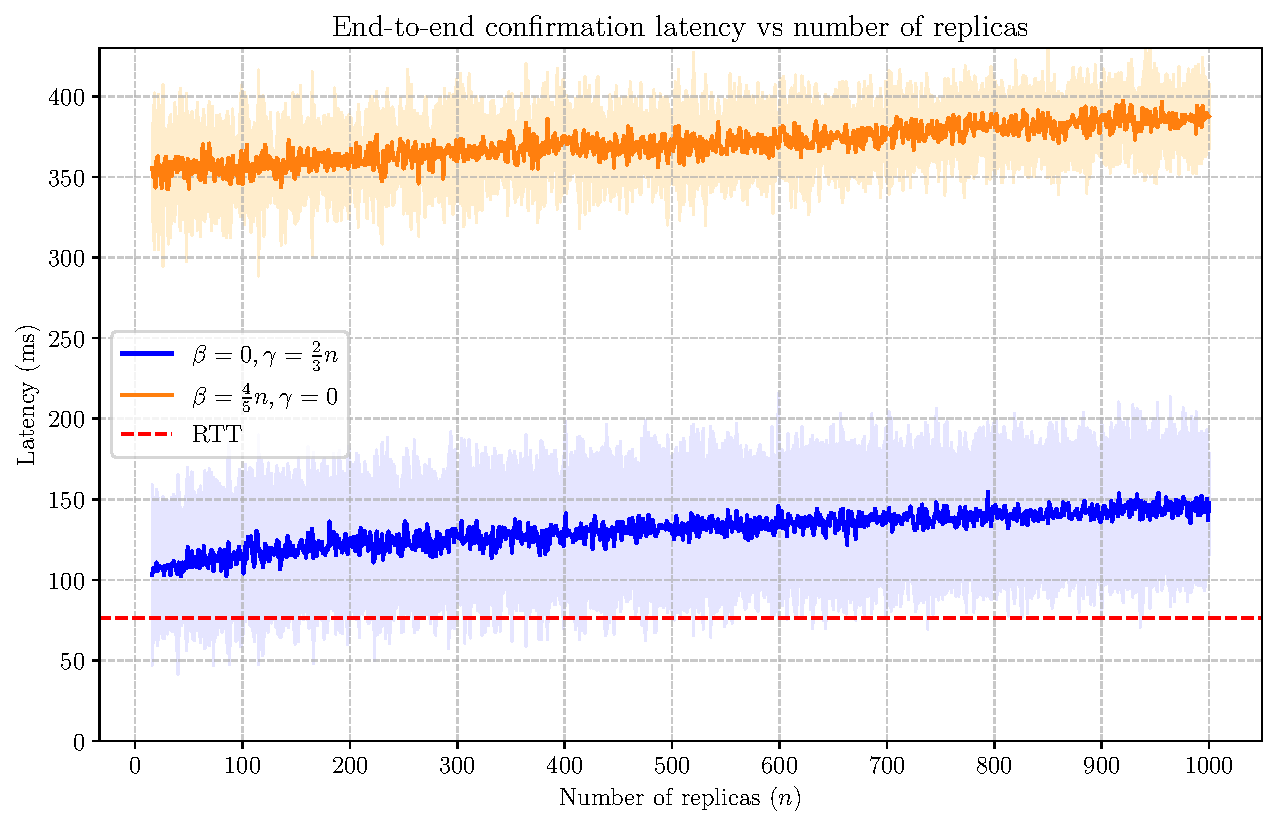
\includegraphics[width=0.9\textwidth]{figures/latency.pdf}
    \caption{End-to-end confirmation latency from a writing client to a reading client as a transaction traverses across $n = 15, \ldots, 1000$ replicas,
    for two reading clients:
    (1) a client that expects up to $\gamma = \lceil\frac{1}{3}n\rceil$ omission faults (blue line, below), and (2) a client that expects up to $\beta = \lceil\frac{1}{5}n\rceil$ Byzantine faults (orange line, above).
    We also plot the physical network round-trip time (RTT) between the reading client and the writing client, which is 76ms (dashed red line).
    A 95\% confidence interval is shown for each experiment (shaded area).}
    \label{fig:latency}
\end{figure}

To validate our theoretical results regarding optimal latency in Pod, we implemented a prototype in Rust 1.85. 
Our implementation consists of both replica and client code. The purpose of the prototype is to measure the 
end-to-end confirmation latency of a transaction from the moment it is sent by the writer client until it is 
confirmed by the reading client. We show the result in \Cref{fig:latency}.


The implementation follows a client-server architecture where each replica maintains two TCP listening sockets: 
one for the reading client connection and one for the writing client connection. Upon receiving a transaction 
payload from a writer, the replica creates a tuple containing the payload, a sequence number, and the current local timestamp.
The replica then signs this tuple using a Schnorr signature (on the secp256k1 curve), appends it to its local ledger, and forwards 
the signed tuple to the reading client.

The system involves two types of clients. The writing client establishes connections to all replicas, records
the timestamp (in its local view) right before sending the transaction and sends transaction 
payloads to each connected replica. The reading client maintains connections to all replicas, validates incoming signed 
transactions, and records the timestamp (in its local view) upon receiving a quorum of valid signatures for a particular transaction.

We conducted experiments with two different quorum sizes: $\beta = \lceil\frac{2}{3}N\rceil$ for omission fault tolerance 
and $\beta = \lceil\frac{4}{5}N\rceil$ for Byzantine fault tolerance. Additionally, we repeated the experiments for 
different numbers of replicas ($N = 15, \ldots, 1000$). The latency is computed as the difference between the timestamp 
recorded by the reading client upon seeing quorum and the initial timestamp recorded by the writing client. 
We repeated each experiment five times and used the mean latency as the final result.

To automate the deployment process, we dockerized the replica binary into a single image shared across all replicas. 
The deployment process begins by launching replicas using a round-robin strategy across seven 
AWS regions: eu-central-1 (Frankfurt), eu-west-2 (London), us-east-1 (N. Virginia), us-west-1 (N. California), 
ca-central-1 (Canada), ap-south-1 (Mumbai), and ap-northeast-2 (Seoul). Each replica is deployed on a 
t2.medium EC2 instance (2 vCPUs, 4GB RAM) and is initialized with user data that contains 
the replica's unique secret signing key. After collecting all replica IP addresses and public keys, we deploy the reading 
client in eu-west-2 (London) and the writing client in us-east-1 (N. Virginia), both initialized with the complete 
list of replica information (ip addresses and public keys).

The entire deployment process is fully automated using the AWS SDK for Rust (aws-sdk-ec2 v1.17.0).
The process handles instance creation, security group configuration, and user data initialization.
creation, security group configuration, and user data initialization. This enables us to scale
up to 1000 replicas with a single command.

As shown in Figure~\ref{fig:latency}, our experimental results demonstrate that the latency remains largely independent 
of the number of replicas. We observe that due to the quorum size, the reader achieves quorum as soon as the fastest 
$\beta$ replicas have responded, which gives rise to the happy artifact that the 1 - $\beta$ slowest proportion of replicas
do not slow down confirmation. As illustrated in Figure~\ref{fig:latency}, the confirmation latency 
fluctuates around 112ms for the omission fault experiment and around 141ms for the Byzantine experiment. Which approximates
the physical network RTT between the reading client and the writing client that stands at 76ms.
